\chapter{Problématique de la détection}
	\section{Généralités}

Les techniques de comparaisons d'organes de décision types ROC (Receiver-Operating Curve) proviennent à l'origine du domaine des télécommunications. Il fallait une métrique permettant de tester les performances des systèmes RADAR\cite{zou2007receiver}.

Les courbes \ROC servent donc à évaluer la capacité de un ou plusieurs ``observateurs'' à discriminer des signaux entre deux classes. On utilise habituellement les informations de sensibilité et de spécificité pour l'évaluation

Les techniques que j'ai utilisé par la suite pour comparer les performances des algorithmes de correction du mouvement respiratoire sont basées sur les courbes \ROC, ou Receiver-Operating Curves. Elles ont été utilisées en médecine à partir de ... (1978 publi FROC, voir pour ROC)

Les performances d'un classifieur sont indiquées par la matrice de confusion, qui recense les signaux correctement et incorrectement classés 

\begin{tabular}{cc c|c|}
	
	& & \multicolumn{2}{c}{Classe estimée} \\
	\cline{3-4}	
	& & \multicolumn{1}{|c|}{Sain} & pathologique \\ 
	\cline{2-4}
	\multicolumn{1}{c|}{\multirow{2}{*}{Classe réelle}} & \multicolumn{1}{|c|}{Sain} & VN (\emph{Vrai Négatif}) & FP (\emph{Faux Positif})\\
	\cline{2-4}
	\multicolumn{1}{c|}{} & \multicolumn{1}{|c|}{Pathologique} & FN (\emph{Faux Négatif}) & VP (\emph{Vrai Positif})\\
	\cline{2-4}
\end{tabular}


On utilise habituellement deux grandeurs pour mesurer les performances d'un classifieur :

La \emph{sensibilité} (eq. \ref{eq:sensib}) correspond à la proportion d'images correctement évaluées pathologiques par l'observateur par rapport au nombre total d'images réellement pathologiques. Elle donne une information sur la capacité du classifieur à détecter les cas pathologiques.

\begin{equation}
	\label{eq:sensib}
	Sensibilite = \frac{VP}{VP + FN}
\end{equation}

La \emph{spécificité} (eq. \ref{eq:specif}) représente le même type de grandeur, mais cette-fois ci appliquée aux cas non pathologiques : elle correspond à la capacité du test à donner un résultat négatif lorsque l'image est non pathologique.

\begin{equation}
	\label{eq:specif}
	Specificite = \frac{VN}{VN + FP}
\end{equation}

Ces deux grandeurs sont complémentaires mais ne permettent pas à elle seules de comparer des classifieurs. En effet, un  utilisteur va plutôt donner des notes (voir papier sur gradation tumeurs mammaires)

	\section{Méthodologie \ROC - Receiver-Operating Curve}

Les \ROC sont des courbes indiquant la spécificité et la sensibilité du modèle de classification pour différents niveaux de certitudes. Elles fournissent une mesure objective des performances d'un observateur dans une tâche de discrimination entre deux classes. 

l'évaluation d'un observateur par la méthode ROC implique de créer un jeu de données de données labellisé en deux classes : Normale (H0) et Pathologiques (H1). L'observateur va se voir présenter l'ensemble des images et devra décide pour chacune si elle est H1 ou H0. Cela se fait en donnant une note (notée $\lambda$) : plus elle sera élevée, plus l'observateur va considérer qu'il est en présence d'un cas pathologique. A l'inverse, une note basse va indiquer un cas présumé sain.

Le tracé de la courbe \ROC se fait en reportant la sensibilité et la spécificité du classifieur pour différentes notes. Par construction, la courbe va commencer au point $(0,0)$ et se terminer au point de coordonnée $(1,1)$

\begin{figure}[h]
	
	\label{fig:courbeROC}
	\begin{center}
	\includegraphics[width=10cm]{images/courbeROC}
	\end{center}
	\caption{la courbe ROC indique la sensibilité et la spécificité pour chaque niveau de confiance. L'aire sous la courbe ROC est un indicateur de la performance du classifieur.}
\end{figure}

Le formalisme \ROC considère que les distributions de probabilité des faux positifs et des vrai positifs suivent une loi gaussienne -voir fig. \ref{fig:loiROC}

\begin{figure}[h]
	
	\label{fig:loiROC}
	\begin{center}
	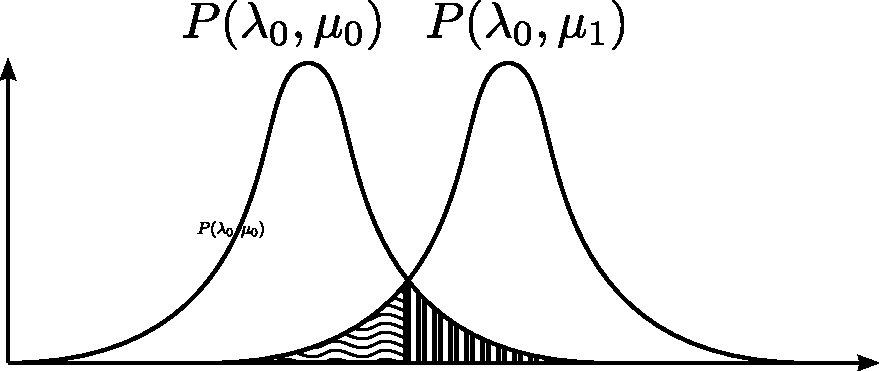
\includegraphics[width=10cm]{images/loiROC}
	\end{center}
	\caption{Loi \ROC}
\end{figure}

Un ensemble d'indicateurs permettent de comparer les performances de classifieurs à partir des courbes ROC. Le plus simple consiste à choisir un niveau de spécificité et à comparer les sensibilités des classifieurs. L'aire sous la courbe ROC est elle aussi très utilisée \cite{nie2006integrating}. 

$p$-valeur ?

Le problème de cette technique est que l'observateur ne donne pas d'information de localisation du problème dans l'image. Dans notre cas, nous voulons comparer des classifieurs qui détectent les tumeurs dans l'image. Il faut non seulement savoir si des lésions sont présentes, mais aussi avoir leur nombre et leur localisation. Cela est plus proche du travail en routine clinique qui consiste à évaluer l'étendue et le nombre des lésions pour déterminer l'efficacité d'un traitement par exemple. 

Pour éviter cette limitation, plusieurs extensions à la méthodologie \ROC sont décrites dans la littérature. Celle qui correspond le plus à nos besoins (multi site, multi lésions) est la courbe \FROC.

	\section{\FROC}	

les courbes \FROC sont une généralisation des courbes \ROC aux cas où l'observateur ne connaît à priori ni le nombre ni la localisation des lésions dans l'image. Il doit indiquer un ensemble de lésions potentielles dans l'image et associer à chacune une note.

Dans ce cas, on ne peut pas utiliser le formalisme \ROC car le terme de specificité n'est pas directement calculable pour chaque niveau de confiance. On utilise à sa place le nombre moyen de faux positifs par image pour un seuil donné (voir fig.\ref{fig:courbeFROC}).

\begin{figure}[h]
	
	\label{fig:courbeFROC}
	\begin{center}
	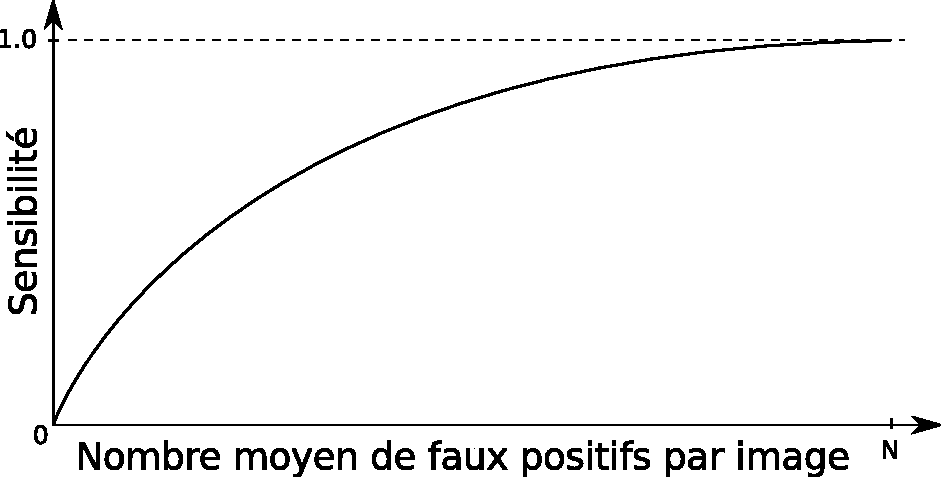
\includegraphics[width=10cm]{images/FROC}
	\end{center}
	\caption{Courbe \FROC}
\end{figure}

Les courbes F-ROC n'ayant pas de bornes sur l'axes des abscisses, il est impossible de 

\chapter{Systèmes de détection}

	\section{Les CAD en TEP}

Plusieurs systèmes d'assistance au diagnostique pour l'imagerie médicale ont été développés depuis  

	\section{Types de classification}
		\subsection{supervisée - méthodologie}

Les classifieurs supervisés nécessitent une connaissance a priori des classes. On entraîne le classifieur en lui fournissant des \emph{exemples} de cas avec l'étiquette associée. A partir de cette base de données d'entraînement, le classifieur va générer un \emph{modèle} predictif permettant de classer de futurs exemples non encore connus.

\begin{figure}[h]
	
	\label{fig:courbeFROC}
	\begin{center}
	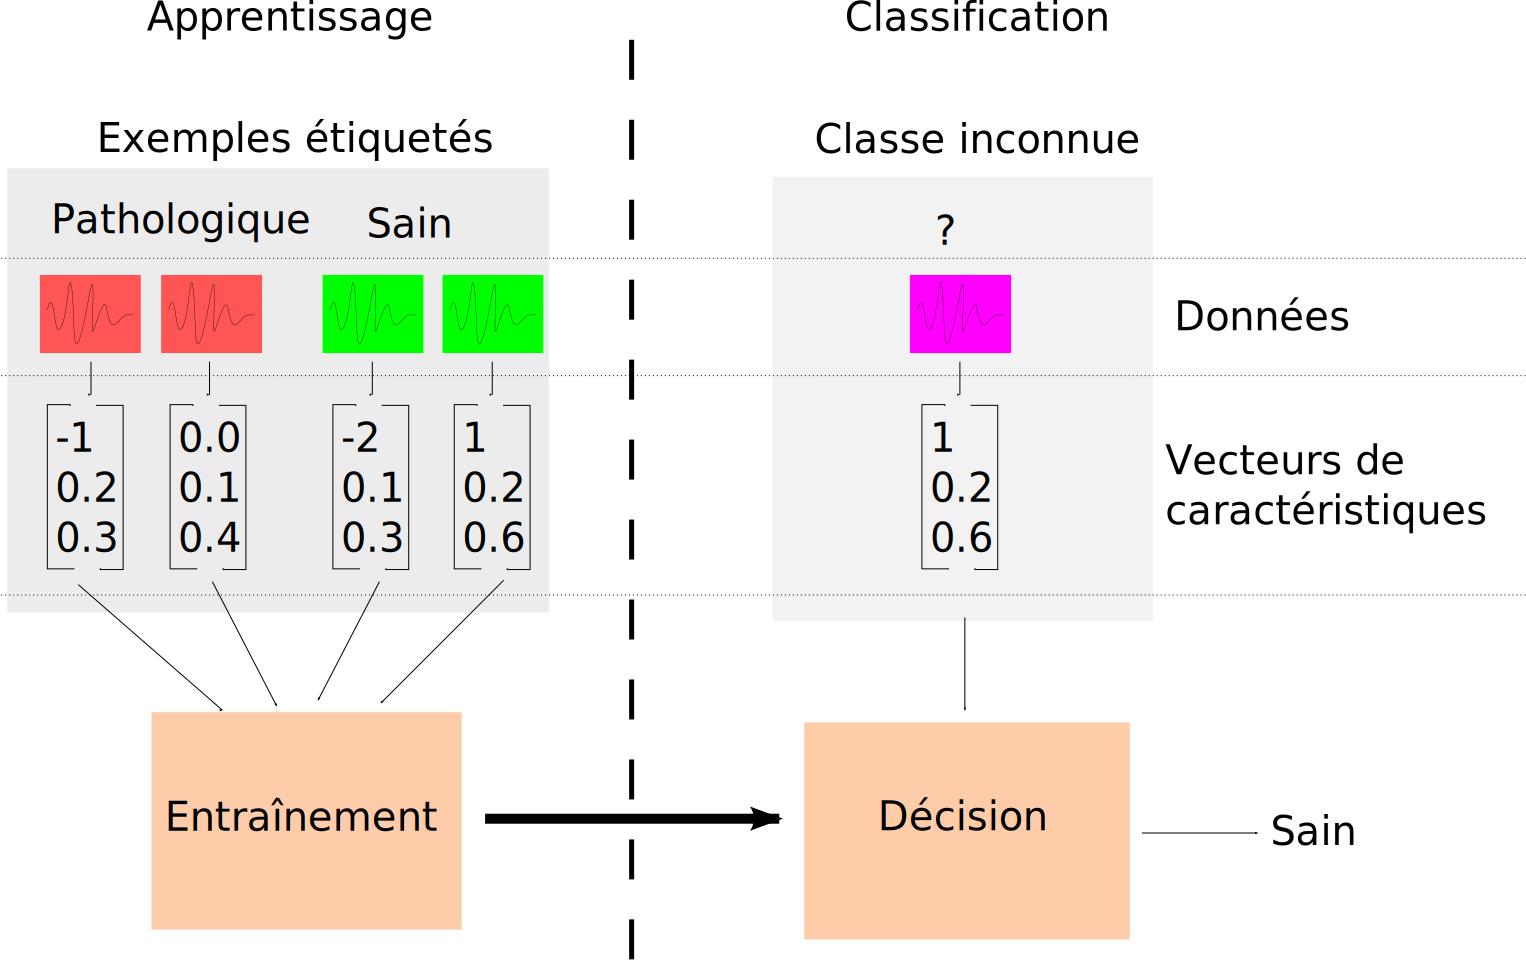
\includegraphics[width=15cm]{images/fonctionnementClassif}
	\end{center}
	\caption{Courbe F-ROC}
\end{figure}

		\subsection{non supervisée - méthodologie}

Dans le système de classification non supervisé, on fourni directement au classifieur l'ensemble des données à traiter. Il devra de lui-même les classer par similitude en groupes. On utilise ce type de classifieur si on ne connaît pas a priori les classes.

	\section{classifieurs}

		
		\subsection{SVM (Separateur à Vaste Marge)}

Ce type de classifieur se base sur 
		\subsection{LDA}

	\section{Systèmes humain}
	% besoin d'avoir des données fiables ?